\documentclass[a3paper, 12pt]{article}
\usepackage[utf8]{inputenc}
\usepackage[spanish]{babel}
\usepackage[top=2cm, left=2cm]{geometry}
\usepackage{amsmath, amssymb, amsfonts, latexsym}
\usepackage{graphicx}
\usepackage{xcolor}
\usepackage{multicol}
\usepackage{nicefrac}

\author{Andrea Chumaña}
\title{Deber Capitulo 6}
\date{\today}


\begin{document}
\maketitle
La solución de la ecuación diferencial
\begin{center}
  \begin{equation*}
y^{'} + 2y(x)= \left\lbrace
\begin{array}{ll}
\text{1} & \text{si} \quad x\in [0,3],\\
\text{0} & \text{si} \quad x > 3.
\end{array}
\right.
\end{equation*}
\end{center}
{\color{magenta}Está dada} por la función a trozos 
\begin{center}
 \begin{equation*}
y(x)= \left\lbrace
\begin{array}{ll}
\dfrac{1}{2}(\exp^{-2x}-1)& \text{si} \quad x\leq 3,\\
\\
\dfrac{1}{2}(\exp^{-2x}-\exp^{6-2x)}& \text{si}  \quad x > 3.
\end{array}
\right.
\end{equation*}
\end{center}
\begin{figure}[h!] 
\centering 
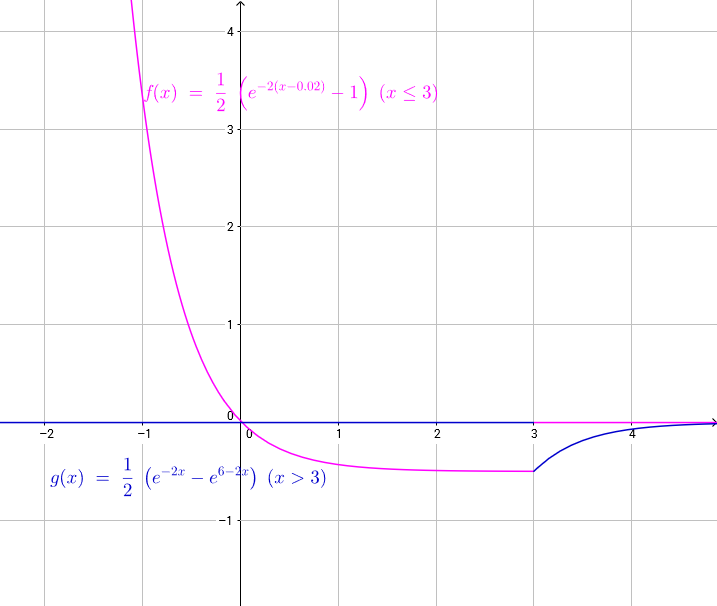
\includegraphics [scale = 0.5]{grafico1}
\caption{ \emph{<<Funciónes a trozos>>}.}
\label{mec} 
\end{figure}
\end{document}